\aufgabenteil{a)}
Der Zweigüberdeckungstest ist stärker, da nicht nur alle Anweisungen ausgeführt werden, sondern auch alle möglichen Entscheidungen
(false \& true) durchlaufen werden. Hier kann sich herausstellen, dass manche Verzweigungen nie benutzt werden und somit eine unnötige
Abfrage darstellen. 


\aufgabenteil{b)}
Die folgende Funktion soll das Vorzeichen des übergebenen Parameters berechnen. Für eine Eingabe $x$ sei $f(x)$ wie folgt
definiert:
\begin{center}
$f(x) = \begin{cases}
	1,   & \text{falls } x > 0 \\
	-1,   & \text{falls } x < 0\\
	0,   & \text{falls } x = 0
\end{cases}$ \\
\end{center}
Nun die Methode f mit einem kleinen Fehler:
\begin{lstlisting}[language=Java]
     public int f(int x){
1: 	int res = 42;
2:      if(x<0){
3:         res = -1;
4:      } else if(x>0) {
5:         res = 1;
        }
6:	return res;
     }
\end{lstlisting}
\begin{figure}[h]
  \centering
  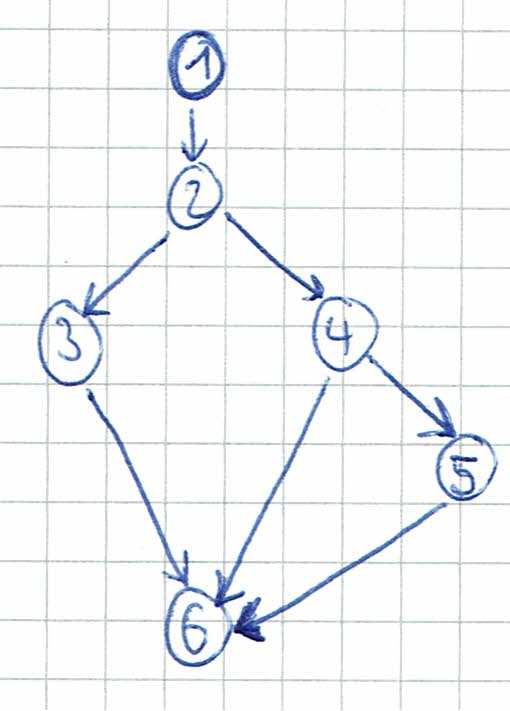
\includegraphics{3b_cont.jpg}
\end{figure}
\begin{enumerate}
\item Testfall: $x=-2$, überdeckt Anweisungen 1,2,3,6
\item Testfall: $x=2$, überdeckt Anweisungen 1,2,4,5,6
\end{enumerate}
Zusammen erhält man eine volle Anweisungsüberdeckung, auf den Testeingaben
erhält man die erwarteten Ergebnisse. Bei der Anweisungsüberdeckungstest
fällt also der Fehler, dass die Methode bei Eingabe 0 ein falsches Ergebnis
ausgibt, nicht auf. \\
Erst ein Zweigüberdeckungstest würde den Fehler aufzeigen, da so noch der
implizite else-Teil, in welchem x==0 wäre, betrachtet wird. Für einen
Zweigüberdeckungstest könnte man dann die Eingaben der beiden Testfälle aus dem 
Anweisungsüberdeckungstest übernehmen und noch zsätzlich einen dritten Testfall
mit $x=0$ einführen, bei welchem auffällt, dass das Ergebnis 42 ist, also
nicht das erwartete Ergebnis 0.

\aufgabenteil{c)}
Die folgende Methode posTimesTwo soll als Eingabe einen int x bekommen, und das Zweifache von
x zurückgeben, jedoch soll das Ergebnis strikt positiv, also immer echt größer 0 sein, weshalb 
bei negativen Eingaben zuerst mal -1 gerechnet wird.\\
Der Fehler im Programm liegt darin, dass die 0 nicht richtig berücksichtigt wurde, kommt zu einer Endlosschleife,
jedoch sollte das Programm terminieren und die Rückgabe stets strikt positiv sein, zum Beispiel könnte man für die Eingabe 0 den Wert 1 returnen.
\begin{lstlisting}[language=Java]
     public int posTimesTwo(int x){
1:      int y=x;
2:      while(true){
3:         if(y<=0){
4:            y=(-1)*y;
           } else {
5:            y=y*2;
6:            break;
           }
        }
7:      return y;
     }
\end{lstlisting}
Der Kontrollflussgraph sieht wie folgt aus:\\
\begin{figure}[H]
  \centering
  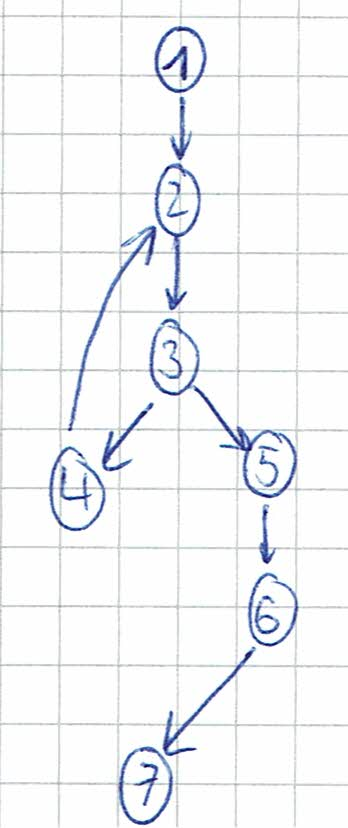
\includegraphics{3c_cont.jpg}
\end{figure}\ \par
Bereits mit einer Eingabe < 0 erreicht man schon eine Zweigabdeckung, zum Beispiel der Eingabe -1. Es ergibt sich die Abarbeitungsfolge 1,2,3,4,2,3,5,6,7.
Dabei werden alle Zweige im Kontrollflussgraphen besucht und man erhält das korrekte Ergebnis 2.\par
Bei einem Pfadabdeckungstest sieht dies anders aus: Man muss sich zunächst überlegen, welche Pfade möglich sind. Einmal wäre der Pfad aus dem Zweigabdeckungstest
möglich, außerdem noch der Pfad 1,2,3,5,6,7 für eine Eingabe > 0, zum Beispiel 1. Dabei wird das Ergebnis 2 geliefert, dies ist ok. \\
Nun ist aber noch ein dritter Pfad möglich, nämlich für die Eingabe 0, dieser sieht so aus: 1,2,3,4,2,3,4,... , wobei sich 2,3,4 periodisch wiederholt und eine
Endlosschleife vorliegt, welche vom Zweigabdeckungstest nicht zwingend gefunden wird. Somit ist die Pfadabdeckung mächtiger.